\documentclass[12pt]{article}
\usepackage[pdftex]{graphicx}
\usepackage{epstopdf}
\usepackage{amsmath, algorithmic, color, multicol}
\usepackage{subfigure}


\title{Answers to Problem Set 3}
\author{
	Lauren Hinkle (lhinkle)\\
	Pedro d'Aquino (pdaquino)\\
	Robert Goeddel (rgoeddel)}

\begin{document}
\maketitle
\pagebreak

%% TASK 1
\section{FastSLAM}

% PART A
\paragraph{A}
Starting with an existing EKF with state $\left[\begin{array}{c c c c c}x_0 & y_0 & t_0 & fx_0 & fy_0\end{array}\right]$ and a corresponding covariance matrix $\Sigma$.
\subparagraph{i}
For our first observation, we merely add our estimated position for the observation
directly to the mean/state vector based on our current position estimate and the
observation values $r$ and $\phi$. This gives us:

$$x' = \left[\begin{array}{c}x_0 \\
        y_0 \\
        \theta_0 \\
        fx_0 \\
        fy_0 \\
        x_0 + r \cos (\theta_0 + \phi) \\
        y_0 + r \sin (\theta_0 + \phi)
        \end{array}\right]
$$

To calculate the covariance, we need to base our uncertainties for our new observation
on the uncertainties of all we've seen before and the uncertainties introduced by taking
the observation itself. We use the formula:

$$\Sigma_w = \left[\begin{array}{c c}
    3 & 0 \\
    0 & 1 \end{array}\right]
$$

$$\Sigma'_x = J^f_x \Sigma_x (J^f_x)^T + J^f_w \Sigma_w (J^f_w)^T$$

$$f(x, y, \theta, r, \phi) = \left[\begin{array}{c}
    x + r\cos(\theta+\phi) \\
    y + r\sin(\theta+\phi) \end{array}\right]$$
    
$$r = r + \omega_r$$
$$\phi = \phi + \omega_\phi$$

In this case, $\Sigma_x$ is our old covariance and $\Sigma_w$ is our observational covariance.
$J^f_x$ is a $7 \times 5$ matrix in this case consisisting of the identity for the first 5 rows (preserving
the original entries) and then the Jacobian of the function $f$ with respect to the state vector variables,
at the current state estimate. $J^f_w$ is the $7 \times 2$ Jacobian of $f$ with respect to the noise variables $\omega_r$ and $\omega_\phi$.

The result is a $7 \times 7$ covariance matrix. The intution for this equation is that there are two sources
of uncertainty for the estimate of the new feature. The first term, $J_x\Sigma_xJ_x$, is accounting for the
covariance that comes from the uncertainty in the estimate of the current robot pose. This makes sense: even
if we had a perfect observation, there would still be some uncertainty in the feature position unless we were
also completely sure about the current pose. The second term adds to the covariance matrix the error that came
from the observation itself. In this case, the sensor noise is additive so the Jacobian is essentially performing a projection
from $(r, \phi)$ space into $(x, y)$. If we had, for example, a proportional noise model, the sensor equations would
change and so would $J_w$.

\subparagraph{ii}
After re-observing $f_1$, the mean and covariance matrix are calculated using an updated Kalman gain (\emph{Note: additional primes denote
    later state}).
$$K' = \Sigma_x' J_{x'}^T(J_{x'} \Sigma_x' J_{x'}^T + \Sigma_w)^{-1} $$
$$x'' = x' + K'r'$$
$$\Sigma_x'' = (I - K'J_{x'}) \Sigma_x'$$

$J_{x'}$ denotes the Jacobian as position $x'$, so a Jacobian in terms of our previous state, but this time we
are projecting  back to $(r, \theta)$. In other words, this Jacobian is exactly like those used in PS2.

\subparagraph{iii}
After observing $f_1$: \\
$$x' = \left[ \begin{array}{c}
3 \\
2 \\
\pi \\
12 \\
15 \\
3 \\
-8
\end{array}\right],
\Sigma'_x = \left[ \begin{array}{c c c c c c c}
     4   &  1  &   2  &   1   &  1  &  24  &   1\\
     1   &  6  &   3  &   1   &  2  &  31  &   6\\
     2   &  3  &   4  &   1   &  2  &  42  &   3\\
     1   &  1  &   1  &   8   &  1  &  11  &   1\\
     1   &  2  &   2  &   1   & 10  &  21  &   2\\
    24   & 31  &  42  &  11   & 21  & 544  &  31\\
     1   &  6  &   3  &   1   &  2  &  31  &   9

\end{array}\right]$$

after re-observing $f_1$:

$$\mu'' = \left[ \begin{array}{c}
    3.0000\\
    2.0000\\
    3.1416\\
   12.0000\\
   15.0000\\
    4.5708\\
   -8.5000
\end{array}\right],
\Sigma''_x = \left[ \begin{array}{c c c c c c c}
     4.00   &  1.00  &   2.00  &   1.00  &   1.00  &  24.00  &   1.00\\
     1.00   &  6.00  &   3.00  &   1.00  &   2.00  &  31.00  &   6.00\\
     2.00   &  3.00  &   4.00  &   1.00  &   2.00  &  42.00  &   3.00\\
     1.00   &  1.00  &   1.00  &   8.00  &   1.00  &  11.00  &   1.00\\
     1.00   &  2.00  &   2.00  &   1.00  &  10.00  &  21.00  &   2.00\\
    24.00   & 31.00  &  42.00  &  11.00  &  21.00  & 494.00  &  31.00\\
     1.00   &  6.00  &   3.00  &   1.00  &   2.00  &  31.00  &   7.50

\end{array}\right]$$

\subparagraph{iv} Compute the mean and covariance of $f_1$:
$$\mu_0 = \left[ \begin{array}{c}
x_0 + r\cos(\theta_0 + \phi) \\
y_0 + r\sin(\theta_0 + \phi) \\
\end{array}\right]$$
$$J =  \left[ \begin{array}{c c}
cos(\theta_0 + \phi) & -r\sin(\theta_0 + \phi)\\
sin(\theta_0 + \phi) & r\cos(\theta_0 + \phi)\\
\end{array}\right]$$
$$\Sigma_0 = J \Sigma_w J^T$$

\subparagraph{v} Update the landmark mean and covariance given re-observation of $f_1$:
$$K = \Sigma_0J^T\left(J\Sigma_0J^T + \Sigma_w\right)^{-1}$$
$$\mu_1 = \mu_0 + Kr$$
$$\Sigma_1 = (I-KJ)\Sigma_0$$
where $\mu_0$ and $\Sigma_0$ are the mean and covariance before this observation and $\mu_1$ and $\Sigma_1$ are the new mean and covariance.

\subparagraph{vi}
After observing $f_1$: \\
$$\mu_0 = \left[ \begin{array}{c}
3 \\
-8
\end{array}\right],
\Sigma_0 = \left[ \begin{array}{c c}
100 & 0 \\
0 & 3
\end{array}\right]$$

after re-observing $f_1$:
$$\mu_1 = \left[ \begin{array}{c}
4.57 \\
-8.5
\end{array}\right],
\Sigma_1 = \left[ \begin{array}{c c c c c c c}
50 & 0 \\
0 & 1.5
\end{array}\right]$$

% Task 1 part B-D
\paragraph{B}
FastSLAM 1.0 samples new robot positions from a distrubtion taking only
odometry measurements into account. However, it is often the case that
a robot's sensors are more accurate than its odometry and control. FastSLAM 2.0
leverages these accurate observation measurements to its advantage, sampling
new poses based on odometry \emph{and} observation measurements. This prevents
FastSLAM 2.0 from sampling as many low likelihood particles, making it more
efficient.

\paragraph{C}
Our particle resampling method resamples particles whenever a new observation
is made, since this is when the weights change. \footnote{Actually we would only need to resample
after a loop closure, because observing new features does not change the weights. However,
each particle has its own data associations; for every observation some particles would
associate it with previously seen landmarks while others would interpret it as a new landmark.}
We iterate through all particles to sum their weights, and then we draw random values between 0 and
the summed weight to select new particles. To determine which particle to pick,
we iterate through the particles, summing the weights again as we go, and when
the sum is greater than our random value, we return a copy of that particle.

To test for sampling bias, we can easily just sample an excessive amount of
particles and compare the resulting distribution of particles to our
expected distribution. If we sample many, many particles, large differences
in the resulting set of particles compared to our expected set will become
increasingly improbable and thus detectable with a certain confidence.

To approximately compute the expected distribution, we can do the following. First, we normalize the weights
of all particles such that the lowest weight is, say, $w_0=1000$, and then round up all the weights so
that they are integers. There is some precision being lost (e.g. for particles with weights of 1.00000 and
1.00001), but we conjecture that with enough tweaking of $w_0$
the resulting weights would be
a reasonable approximation of the original distribution. Then, we create a new set $S$ and insert $w_i$
copies of every particle $p_i$ into it, where $w_i$ is that particle's weight.

We are then able to test for bias by sampling enough particles from the original distribution
(with non-normalized weights) such that the particle with the lowest weight is sampled $w_0$ times.
If the set of sampled particles is approximately the same as $S$, then the sampling method is correct.

\paragraph{D}
Since every particle is an independent entity, particles that make bad
associations will be killed off during resampling. Therefore, our
expectation is that a particle-based method like FastSLAM can get away
with a fairly poor data association technique like nearest-neighbor
because only good associations will survive. A method like least-squares
SLAM commits to the poor associations it makes and may never recover, so
data association techniques must be ``smarter'' than nearest-neighbor
matching.

\paragraph{E}
The video is attached in email.

We are plotting several lines and points to aid in visualizing the algorithm:
\begin{itemize}
	\item Blue line: ground-truth trajectory.
	\item Yellow line: best estimated trajectory, from the particle with the lowest $\chi^2$.
	\item Green line: best estimated trajectory, after alignment*.
	\item Green stars: ground-truth landmarks.
	\item Small red points: latest robot position estimate from all the particles.
	\item Big red points: estimated landmark positions, from the particle with the lowest $\chi^2$. They are connected by lines to the true position of the respective landmarks.
	\item Yellow points: estimated landmark positions, after alignment*.
	\item Gray points: landmark position estimates for all particles.
\end{itemize}

*We compute the alignment as the RBT between the estimated and true landmark positions.

\paragraph{F}
FastSLAM is easy to implement and does not require very ``intelligent'' data
association techniques to work well. In fact, a big advantage of FastSLAM is
that it is more robust to poor data associations than alternative SLAM
algorithms. Least squares it is more consistent in performance as
there is no random element to the problem. Least-squares also maintains
complete information forever, unlike FastSLAM, so it will not throw away
potentially useful information as FastSLAM does in cases involving particle
depletion. In other words, least-squares is good at loop closures.

FastSLAM is a safe choice in environments where data association is difficult.
If one can afford enough particles, it is probable that a particle that makes
the correct associations and can survive to give a good map. Least-squares SLAM
would likely not recover from a bad association without user intervention. However,
in cases where we are confident in our data association, methods like
least-squares SLAM converge faster due to the preservation of loops. Least-squares SLAM
has also been heavily optimized to the point that it may run at competitive (or better) speeds
with FastSLAM. More importantly, FastSLAM does not scale well in environments where
landmarks are observed infrequently as many more particles, possibly intractable amounts, are necessary get consistently
good solutions. Least-squares SLAM will still produce a good solution in this case.

Progress in optimization (for example, exploitation of sparsity in matrices) of least-squares
SLAM has made it a more viable solution to the SLAM problem. Given the choice of fast
least-squares SLAM and FastSLAM, a fast least-squares SLAM is preferable as it maintains
more complete information and has guarantees on results. Likewise, increased processing
power and advances in data association increase our confidence in our ability to find
good associations in many cases, rendering one of FastSLAM's main remaining benefits
less compelling.

%% Task 2
\section{Line Estimation from Laser Data}

\paragraph{A}Deriving a closed-form expression that computes the MSE:
Given
$$M_x = \displaystyle\sum_i x_i \qquad M_{xx} = \displaystyle\sum_i x_i^2 \qquad q_x = \frac{M_x}{N}$$
$$M_y = \displaystyle\sum_i y_i \qquad M_{yy} = \displaystyle\sum_i y_i^2 \qquad q_y = \frac{M_y}{N}$$
 $$\hat{n} = \left[ \begin{array}{c}
-sin\theta \\
cos\theta
\end{array}\right]$$

\begin{align*} MSE &=  \displaystyle\sum_i \left[\left(x_i - q_x)\hat{n_x} + (y_i - q_y)\hat{n_y}\right)\right]^2\\
&=\displaystyle\sum_i \left[-\left(x_i - \frac{M_x}{N}\right)sin\theta + \left(y_i - \frac{M_y}{N}\right)cos\theta\right]^2 \\
&=\displaystyle\sum_i \left(\left(y_i - \frac{M_y}{N}\right)cos^2\theta \right)
-2\displaystyle\sum_i \left(\left(x_i-\frac{M_x}{N}\right)\left(y_i - \frac{M_y}{N}\right)cos\theta sin\theta\right) \\
 &\qquad+ \displaystyle\sum_i \left(\left(x_i - \frac{M_x}{N}\right)cos^2\right) \\
&= cos^2\theta(M_{yy}-\frac{M_y^2}{N}) - 2cos\theta sin\theta(M_{xy}-\frac{M_xM_y}{N}) + sin^2\theta(M_{xx}-\frac{M_x^2}{N})
\end{align*}

\paragraph{B}
We chose an error threshold $0.03$. This threshold is extremely intolerant of error,
generally ensuring any lines that we \emph{do} merge are indeed good fits. This helps
preserve some of the smaller lines that often merged into long, perpendicular lines
incorrectly.

The error threshold is our total tolerance for line errors in $(x,y)$. The sum of
the distances of errors for all points with regards to the line fit cannot exceed this
threshold. Unfortunately, this is an absolute cutoff, so the longer a line gets,
the less likely we become to merge in even a good point, as it will still contribute
some error. Conversely, short lines are more likely to merge in bad points as they
have some remaining wiggle room in their accumulated error.

A more principled method for selecting such a threshold besides the ``it-looks-pretty-good''
trial-and-error method is to actually learn from a few ground-truthed examples. Select
a random subset of frames and have a human fit lines where they feel they are appropriate.
From this, the most na\"{i}ve method for selecting a threshold is to pick the largest error
of any of the human-identified lines. In principal, the algorithm will tolerate any line
that is at least as good as a human-tolerable line. To get a little smarter, we can
introduce a proportional threshold that also depends on the number of points in the line fit.
We can then use these random, human-truthed samples to learn a formula for this proportion.

Fig.~\ref{fig:line_fits} gives examples of both good and bad line fits. As we can see in the
bad cases, our na\"{i}ve, non-proportional threshold often fits very bad lines to small amounts
of widely separated noise. Accounting for the distance between measurements might also
improve our fits, as evidenced by some line fits across large discontinuities.

\begin{figure}[htb]
\centering
\subfigure[Good example of line fits]{
    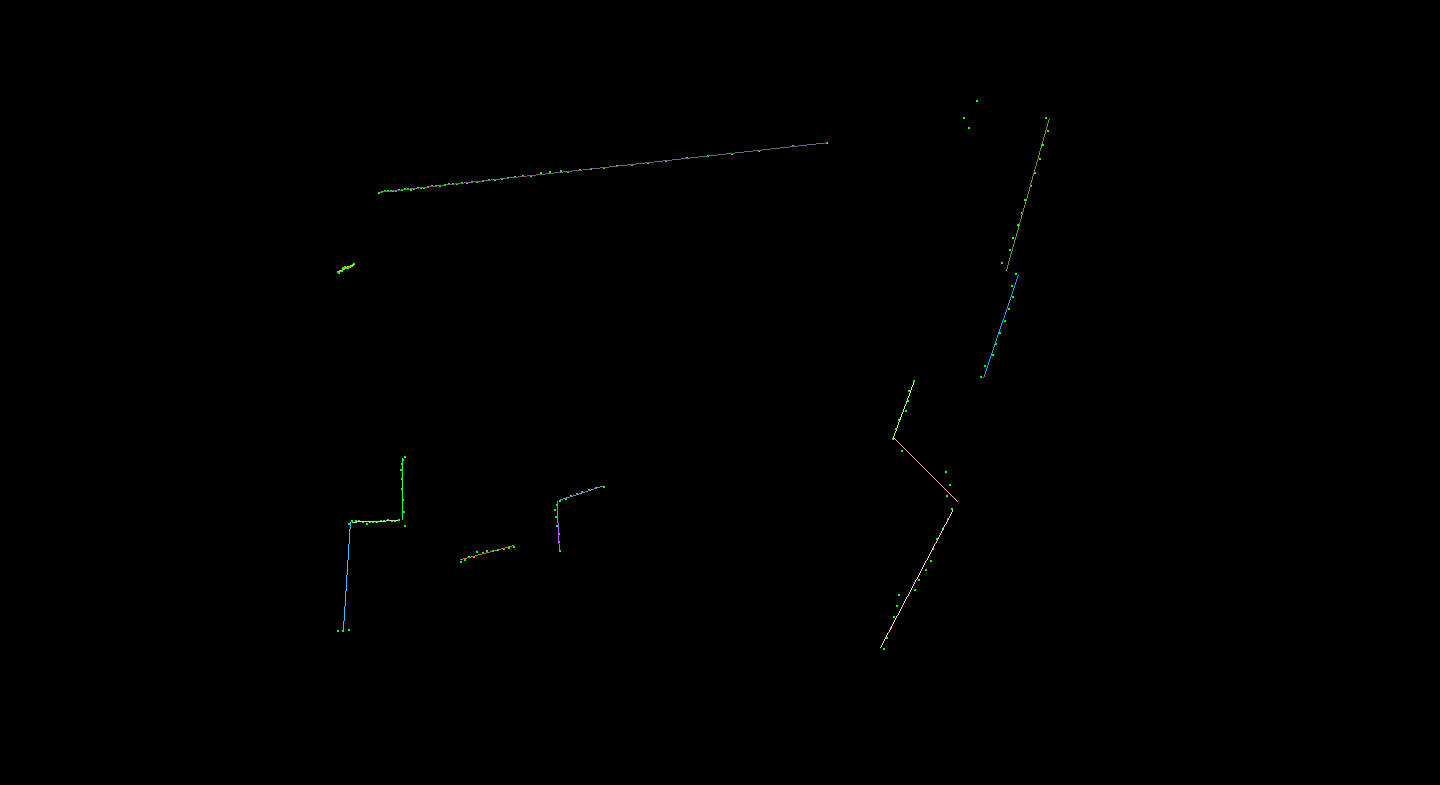
\includegraphics[width=0.7\textwidth]{figures/good_line_fit.png}
    \label{subfig:good_fit}
}
\subfigure[Bad example of line fits]{
    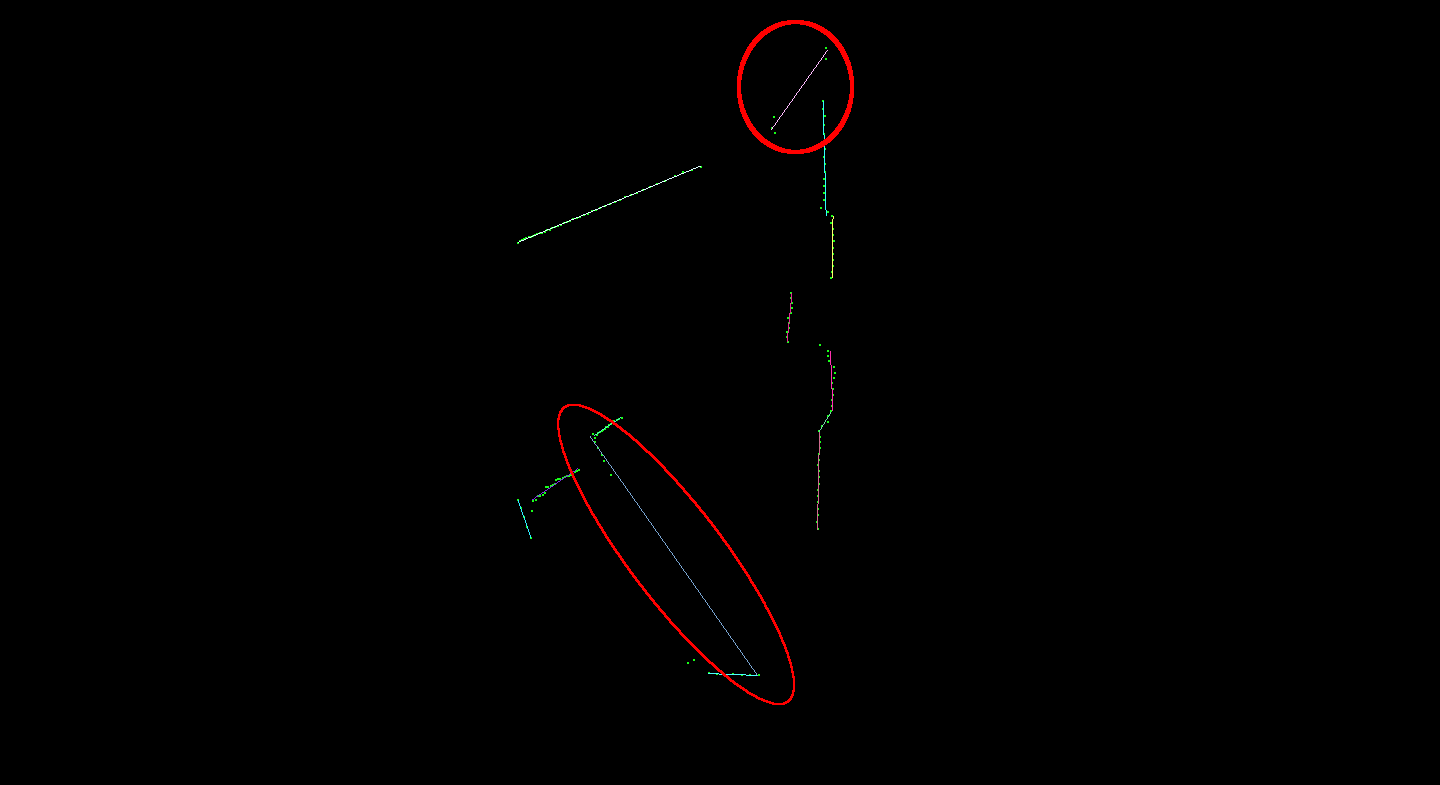
\includegraphics[width=0.7\textwidth]{figures/bad_line_fit_highlighted.png}
    \label{subfig:bad_fit}
}
\caption{Image~\subref{subfig:good_fit} shows a reasonable example of line fits
    extracted using agglomeration. Most lines are fit with quality similar to that
    seen here. However, some lines are fit poorly in cases where there are largeen
    discontinuities. For example, in \subref{subfig:bad_fit} we highlight a pair
    of fits we feel are bad. The line fit to the points in the upper corner, for
    example, is just being fit to two clusters of noise. There is no evidence
    that a line should exist, but the error in merges is small enough that it
    still gets through. The long, circled line starts out as a reasonable fit, but
    makes a large jump to an adjacent point where there is no evidence that such a
    connection should exist.
}
\label{fig:line_fits}
\end{figure}

\paragraph{C}
The idea is to weight fitting errors according to the probability that they came from sensor noise, as opposed to a bad fit. To do that, we project the covariance of the observation from $(r,\theta)$ space to $(x,y)$ and use its inverse as a weight factor in the MSE.

Let $p_i$ be an observation and $q$ a point on the line:

\[MSE = \sum{\left((p_i-q)^T\left(J\Sigma_zJ^T\right)^{-1}\hat{n}\right)^2} \]

Where $\hat{n}$ is a vector normal to the line, $\Sigma_z$ is the observation covariance in $(r,\theta)$ and $J$ is the Jacobian of the function that maps observations in $(r,\theta)$ to the global $(x,y)$ coordinate frame.

This more principled model would make a significant difference when there is a lot of noise.  In this case the original MSE formula might not allow for points to be combined into a line because they are outside a given threshold.  This new calculation for MSE would weight down the seemingly large errors by taking into account that the large difference is more likely.
%% Task 3
\section{RANSAC Rigid-Body Transformation}

\paragraph{A}
Given a number of line correspondences, a set of 3 non-parallel lines that
intersect at unique locations would be sufficient to product a 2D RBT. To
compute the RBT, find the intersections of the lines in each set and then
use Horn's Algorithm to align the resulting sets of 3 points.

\paragraph{B}
Given a fit between lines in set A and lines in set B, we compute a RBT that
rotates A into B's space. To cheaply/quickly compute how good this fit is,
we discretize the world into bins and mark all bins that points from B fall
into. We then apply our transform to the points from A and see if they fall
into a bin from B. If so, we vote $1$, otherwise we vote $0$. The consensus
score is computed as the sum of votes. This is extremely fast as we only need
to bin the points in B once ever and checking for a hit by a point in A only
costs one transformation and a constant time check in a LUT.

After some tuning, we selected a bin size of 10\,cm. This seemed to be a good
balance between ensuring close fits and accounting for the fact that points do
not generally align exactly between scans.

\emph{Disclaimer: The use of a binning method for votes resulted from brainstorming with John Peterson,
    also in the class, about fast ways to calculate votes in such spaces since our existing methods
    were far too slow to use. We can not honestly claim completely that this idea is 100\% ours.}

\paragraph{C}
RANSAC makes good matches much of the time, provided the scans have a reasonable
amount of overlap. Fig.~\ref{fig:good_ransac0} shows how a translation of several
meters is still successfully found by RANSAC. However, eventually this may break
down, even in the presence of human-detectable features, more points will vote
for a bad alignment that ignores these ``good'' and result in the selection of
a sub-optimal transform. This is evident particularly in hallways, where straight,
parallel lines make up the majority of votes and, given the small amounts of overlap in
the optimal match, may vote for poor line matches that. Fig.~\ref{fig:bad_ransac0} gives
an excellent example of this. Finally, Fig.~\ref{fig:long_ransac} shows an example of
RANSAC finding the RBT for two scans that were separated by a significant amount
of travel. These scans were, in fact, of the same location and we were able to extract
a correct alignment from the data.

Our algorithm does not associate lines in real time.  This could be improved upon by
increasing the pre-processing of the lines and using richer features.  This could be done
by improving our line fitting process in Task 2, only using lines with a larger number of
in them, and matching intersections of lines with an angle different of near $\frac{\pi}{2}$.


\begin{figure}[htb]
\centering
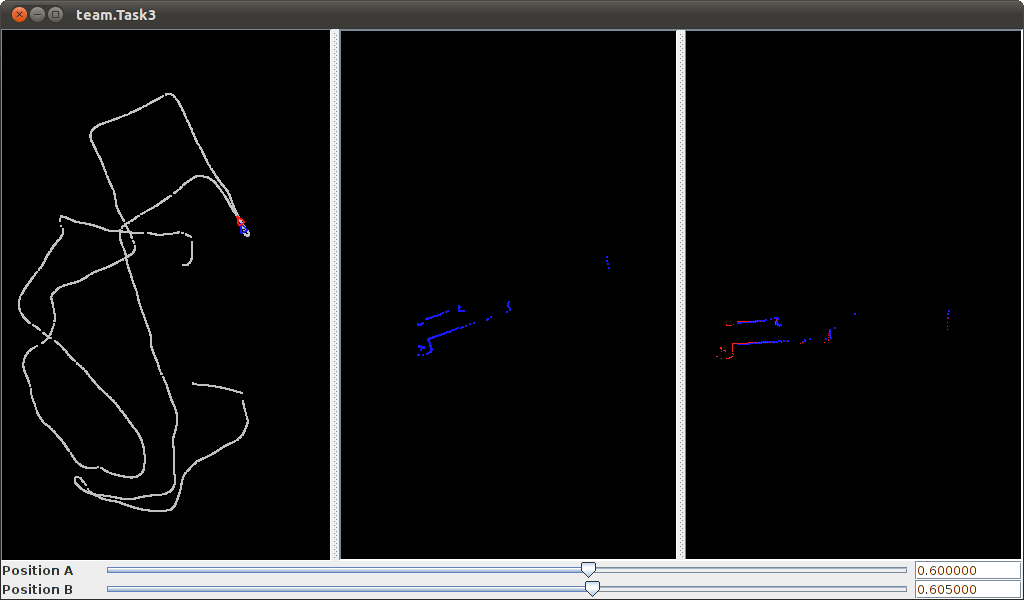
\includegraphics[width=.7\textwidth]{figures/Task3_good0.png}
\caption{A good scan match from RANSAC. Our implementation of RANSAC is able
to fit models to points that are translated or rotated by a non-negligible amount. As seen
in this figure, the recorded poses are separated by several meters, but RANSAC
was able to match features successfully.}
\label{fig:good_ransac0}
\end{figure}

\begin{figure}[htb]
\centering
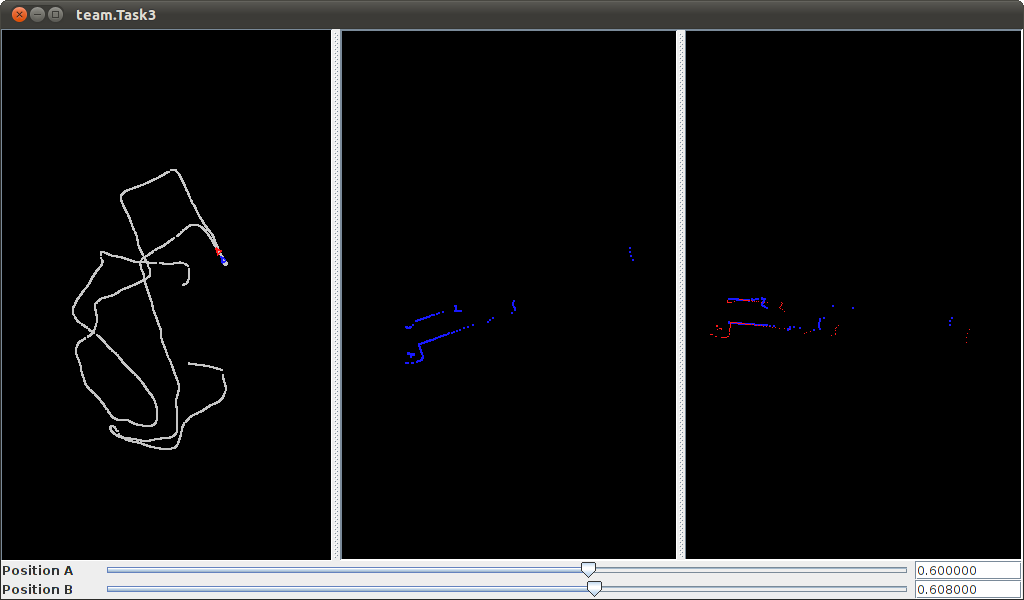
\includegraphics[width=.7\textwidth]{figures/Task3_bad0.png}
\caption{A bad scan match from RANSAC. Eventually RANSAC breaks down because the
    ``good'' features that a human can detect do not hold enough votes to outweigh
    less ``good'' matches. As seen in this figure, after moving the robot slightly
    down the hall from our previously shown good match, RANSAC breaks down and
    returns a significantly less reasonable transformation even though there are
    several features that indicate a good match is still possible.}
\label{fig:bad_ransac0}
\end{figure}

\begin{figure}[htb]
\centering
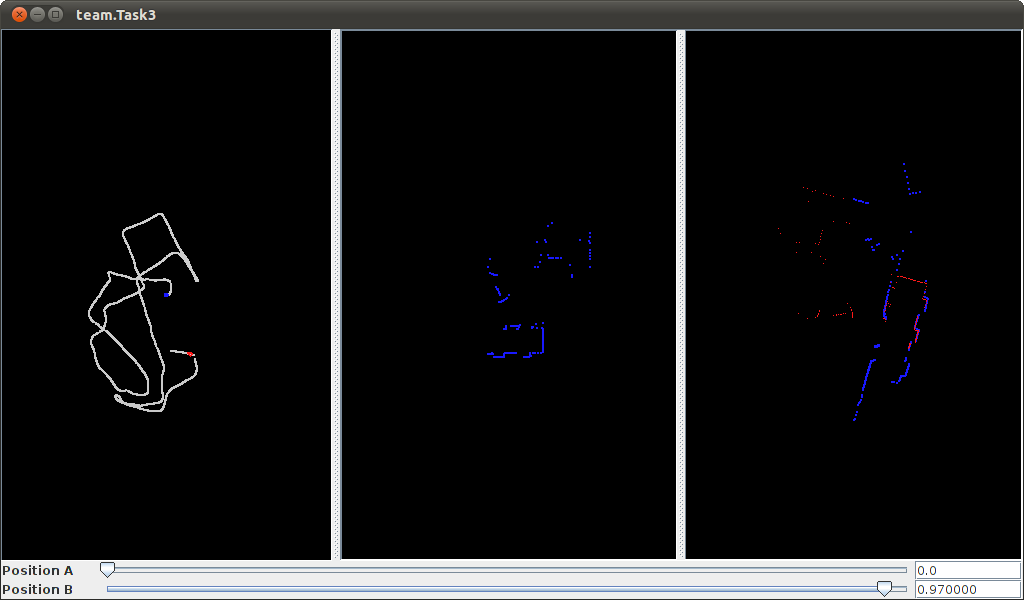
\includegraphics[width=.7\textwidth]{figures/Task3_good_endpoints.png}
\caption{A loop closure detected after significant travel. RANSAC is able to match
    scans when the robot returns to a familiar location after traveling a long
    distance. In this case, the robot starts in an elevator lobby and ends its
    travels in the same elevator lobby. RANSAC is able to detect this, providing a
    RBT that clearly matches the elevator lobby again, though from a different
    perspective.}
\label{fig:long_ransac}
\end{figure}
%% Task 4
\section{Advanced Data Association }
	Data association is the attempt to correlating observed features when we do
not have known data association.  Without good data association, SLAM won't work.
The three ways we have discussed doing data association in class are $\chi^2$
nearest neighbor, RANSAC, and JCBB.

	$\chi^2$ nearest neighbor uses a simple $\chi^2$ to determine whether points
should be associated.  A $\chi^2$ value is determined for associating the new observation
with each previous observation.  The new observation is greedily associated with the previous
observation causing the lowest $\chi^2$ error, unless it is larger than some threshold,
in which case the new observation becomes a new feature.

	The advantage of using $\chi^2$ for data association is that it is simple to implement
and fast to calculate.  However, since $\chi^2$ nearest neighbor's data association is greedy, this can
cause it to miss a good association that is found only by trying to associate a set of features
as a whole.

	RANSAC uses random search to choose a model for associating data points.  Given
a set of new observations, each observation is associated with a random feature, or
becomes a new feature and the resulting $\chi^2$ error is calculated.  This random
association is done several times, and of these iterations, the one with the lowest
resulting $\chi^2$ is chosen as the association for the observations.  RANSAC resolves
the problem $\chi^2$ nearest neighbor falls into of assigning one point at a time greedily.
However, it does not exhaustively search the tree of possible associations, and therefore
does not guarantee finding the ``correct'' association at each new observation.

	In addition to considering multiple points at once, RANSAC is advantageous to more
accurate methods because it is simpler to implement.  An additional advantage of RANSAC
is that it can find associations even when there are many outliers, if it is allowed enough
iterations.  However, the number of iterations to run, as well as the threshold used, change
depending upon the data set.  A ``good'' number of iterations can be calculated, but this doesn't
guarantee finding the best association because RANSAC is probabilistic. RANSAC is also dependent
on the consensus score being cheap to compute. If a cheap score computation does not exist, then
RANSAC loses some of its appeal.
% Doesn't take advantage of points that are ordered

	JCBB seeks to create as few new features as possible (associate as many features
as it can) at each new observation.  It does this by intelligently searching a tree of all
possible associations of the set of new observations.  At each branch, JCBB uses a
heuristic to determine whether to continue searching down the branch for possible
associations or to backtrack and search another branch.  JCBB matches as many features
as it can without causing the $\chi^2$ error to exceed a given threshold.

	Like RANSAC, JCBB typically associates better than $\chi^2$ nearest neighbor because it
considers the effect of assigning multiple associations at once.  An advantage of JCBB
over RANSAC is that it is guaranteed to find the best association of the set of points it is
working with, given an admissible heuristic.  It is, however, harder to implement, and it
depends upon determining an appropriate heuristic for the branch and bound. It also may cost
a tremendous amount as if much pruning is not possible.

In PS2, JCBB or RANSAC would be preferable over nearest-neighbor as our tolerance for
bad associations is low. JCBB, in particular, would guarantee us the highest quality
loop closures and, thus, the best results. If we were concerned about real-time performance,
RANSAC gains appeal as it is fast, but also capable of generating very good associations for
multiple landmarks.

In a project such as FastSLAM (PS3), nearest-neighbor association is sufficient since the
particles that survive resampling should have the best associations. Bad associations will
be thrown out as the solutions are quickly realized to be improbable and are accordingly
weighted very low.
\end{document}
